\documentclass[12pt,a4paper]{article}

% Language setting
\usepackage[portuguese]{babel}
%\addto\captionsportuguese{\newcommand{\andname}{e}}

% Set page size and margins
\usepackage[a4paper,top=2cm,bottom=2cm,left=2.5cm,right=2.5cm,marginparwidth=1.75cm]{geometry}


\usepackage{amsmath}
\usepackage{graphicx}
\usepackage[colorlinks=true, allcolors=blue]{hyperref}
\usepackage{hyperref}
\usepackage{orcidlink}
\usepackage[title]{appendix}
\usepackage{mathrsfs}
\usepackage{amsfonts}
\usepackage{booktabs} % For \toprule, \midrule, \botrule
\usepackage{caption}  % For \caption
\usepackage{threeparttable} % For table footnotes
\usepackage{listings}
\usepackage{enumitem}
\usepackage{chngcntr}
\usepackage{booktabs}
\usepackage{lipsum}
\usepackage{subcaption}
\usepackage{authblk}
\usepackage[T1]{fontenc}    % Font encoding
\usepackage{csquotes}       % Include csquotes
\usepackage{diagbox}


% Customize line spacing
\usepackage{setspace}
\onehalfspacing % 1.5 line spacing

% Redefine section and subsection numbering format
\usepackage{titlesec}
\titleformat{\section} % Redefine section numbering format
  {\normalfont\Large\bfseries}{\thesection.}{1em}{}

% Change the position of the table caption above the table
\usepackage{float}   % for customizing caption position
\usepackage{caption} % for customizing caption format
\captionsetup[table]{position=top} % caption position for tables

% Define the unnumbered list
\makeatletter
\newenvironment{unlist}{%
  \begin{list}{}{%
    \setlength{\labelwidth}{0pt}%
    \setlength{\labelsep}{0pt}%
    \setlength{\leftmargin}{2em}%
    \setlength{\itemindent}{-2em}%
    \setlength{\topsep}{\medskipamount}%
    \setlength{\itemsep}{3pt}%
  }%
}{%
  \end{list}%
}
\makeatother

% Suppress the warning about \@parboxrestore
\pdfsuppresswarningpagegroup=1

%-------------------------------------------
% Paper Head
%-------------------------------------------
\title{PTC3314 - Ondas e Linhas}
\author{2º Exercício de Simulação Computacional}

\affil{Guilherme Fortunato Miranda, Nº USP: 13683786}
\affil{João Pedro Dionizio Calazans, Nº USP: 13673086}
\affil{Thomas de Castro Hess, Nº USP: 11806090}
\affil{Turma 02 – Grupo B}

\date{27 de Outubro de 2024}

\begin{document}

\maketitle

{\begin{center} A tabela de respostas é apresentada ao final do documento, anexadas. \end{center}}

\section{}

\begin{center}
    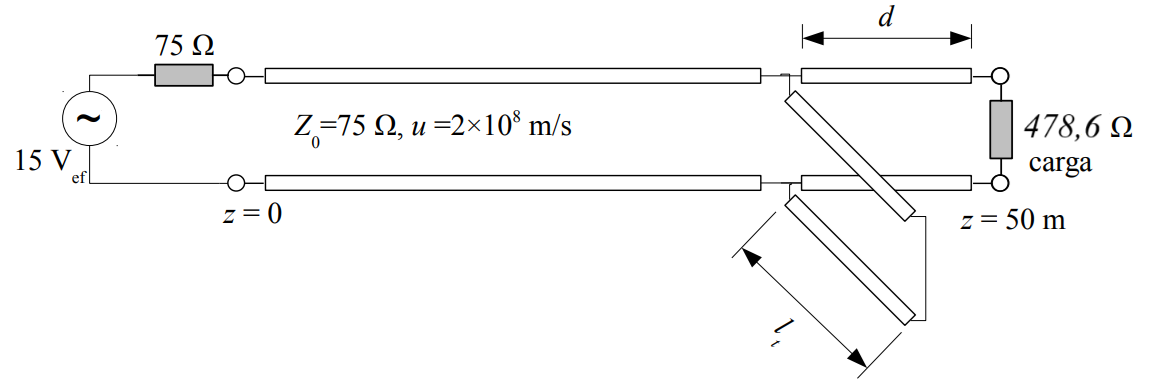
\includegraphics[scale=0.6]{Q1 line.png}
\end{center}

As simulações, gráficos e cálculos para este item foram feitas através do software Octave.

\paragraph{a)}

$P_d = \frac{E_g^2}{4R_g} = 0,75$ W

\paragraph{b)}

$d_{min} = 0,380$ m

$$\rho_d = \rho_L \ e^{-j\frac{4\pi}{\lambda}d}, \ \rho_L = \frac{Z_L - Z_0}{Z_L + Z_0}$$

$$y_d = \frac{Z_0}{Z_d}, \ Z_d = Z_0\frac{1+\rho_d}{1-\rho_d}$$

\paragraph{c)}

$b = 2,13$

\ \ $y_d=1 + jb = 0,9998 + j\ 2,1300 \approx 1 + j\ 2,13$

\paragraph{d)}

$l_t = 0,1397$ m

$$\text{Entrada do toco: } Z_t = \frac{Z_0}{-jb}, \ \rho_t = \frac{Z_t - Z_0}{Z_t + Z_0} = \frac{\frac{1}{-jb} - 1}{\frac{1}{-jb} + 1}$$

$$\text{Final do toco (curto): } Z_{l_t} = 0, \ \rho_{l_t} = 1\angle 180^\circ$$

$$arg\{\rho_t\} = arg\{\rho_{l_t}\} -\frac{4\times 180^\circ}{\lambda}l_t$$

$$l_t = \frac{\lambda}{4}(1 - \frac{arg\{\rho_t\}}{180^\circ})$$

\paragraph{e)} i - Linha sem toco paralelo

$$\rho_{ent}=\rho_L\ e^{-j\frac{4\pi}{\lambda}L}, \ Z_{ent}=Z_0\frac{1+\rho_{ent}}{1-\rho_{ent}}$$

$$I_{ent}=\frac{E_g}{Z_{ent}+R_g}$$

$$P_L=P_{ent}=|I_{ent}|^2R_{ent}$$

\begin{center}
    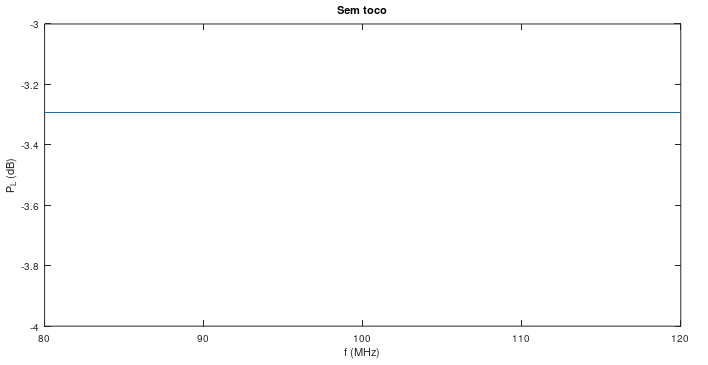
\includegraphics[scale=0.65]{e i.png}
\end{center}

\ \ $P_{max}=P_L\ (cte) =0,35137\ W=-3,29297\ dB$ e BW = 0

\paragraph{e)} ii - Toco localizado em $d_{min}$

Antes do toco:
$$\rho_d^-=\rho_L\ e^{-j\frac{4\pi}{\lambda}d_{min}}$$

Após o toco:
$$Y_d = \frac{1}{Z_0}\cdot \frac{1-\rho_d}{1+\rho_d} - j\frac{b}{Z_0}$$

$$\rho_d^+=\frac{\frac{1}{Y_d}-Z_0}{\frac{1}{Y_d}+Z_0}$$

$$\rho_{ent}=\rho_d\ e^{-j\frac{4\pi}{\lambda}(L-d)}$$

\begin{center}
    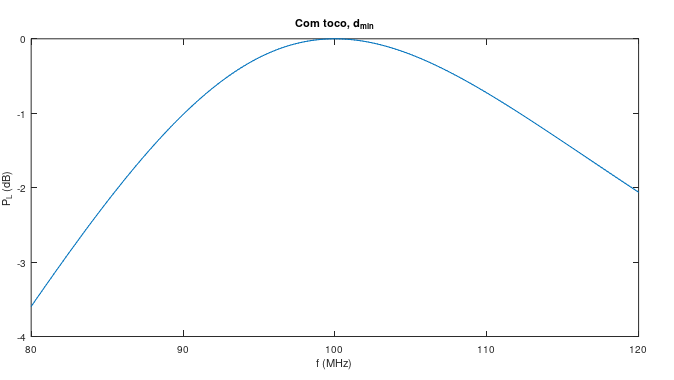
\includegraphics[scale=0.65]{e ii.png}
\end{center}

$P_{max}=P_d=0,75\ W=0\ dB$


BW = de 85,8 MHz a após de 119,6 MHz = 33,8 MHz

\paragraph{e)} iii - Toco localizado em $d_{min}+3m$

\begin{center}
    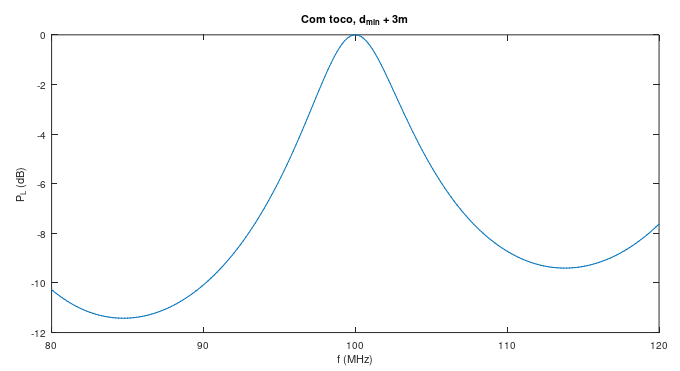
\includegraphics[scale=0.65]{e iii.png}
\end{center}

$P_{max}=P_d=0,75\ W=0\ dB$

BW = de 97,8 MHz a 102,4 MHz = 4,6 MHz

\paragraph{f)} Para valores maiores de d, a largura de banda diminui de valor, em uma taxa menor. Porém, caso o aumento se dê no valor específico do comprimento de onda de cada frequência da amostragem, o valor deve se manter igual ao sem esta parcela múltipla.

$3$ m, por exemplo, tem comportamento equivalente a ($3+\frac{\lambda}{2}$) m, ou até a ($3+9\frac{\lambda}{2}$) m.

Simulações extras para casos condizentes estão apresentadas a seguir.

\vspace{1.5cm}

\begin{center}
    \begin{figure}[h]
    \hspace{-55pt}
    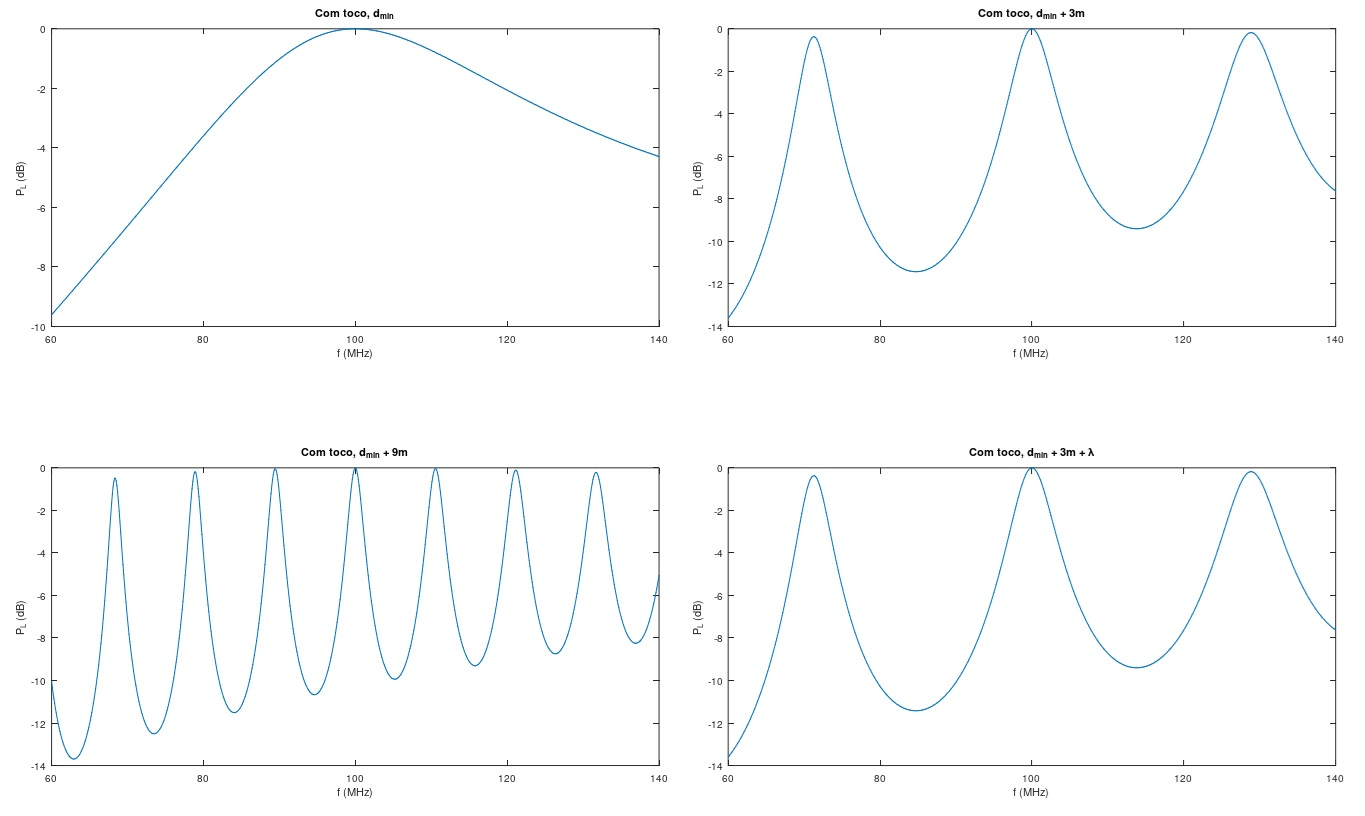
\includegraphics[width=1.24\textwidth]{estendidas.jpg}

    \caption{Simulações adicionais da questão 1}
    \label{fig:awesome_image}
    
    \end{figure}
\end{center}

%-------------------------------------------
%-------------------------------------------
\newpage
\section{}

\begin{center}
    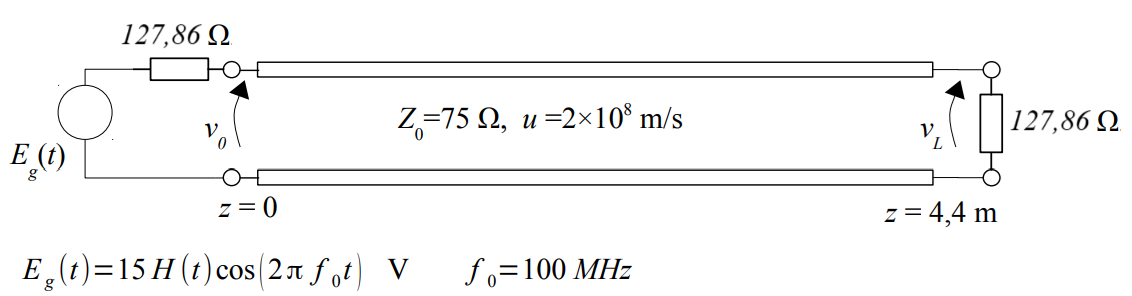
\includegraphics[scale=0.6]{Q2 line.png}
\end{center}
\ \ $Z_g=Z_L=127,86\ \Omega$
\begin{center}
    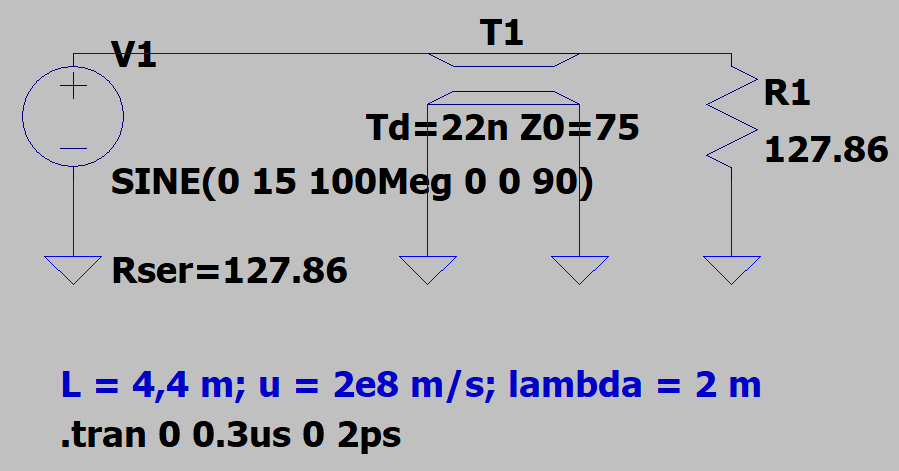
\includegraphics[scale=0.6]{Q2 simu.png}\\
    
    \small{Linha simulada através do software LTspice}
\end{center}

\paragraph{a)}

\begin{center}
    $v(t,z=0),\ 0 < t < 0,3 \mu s$
    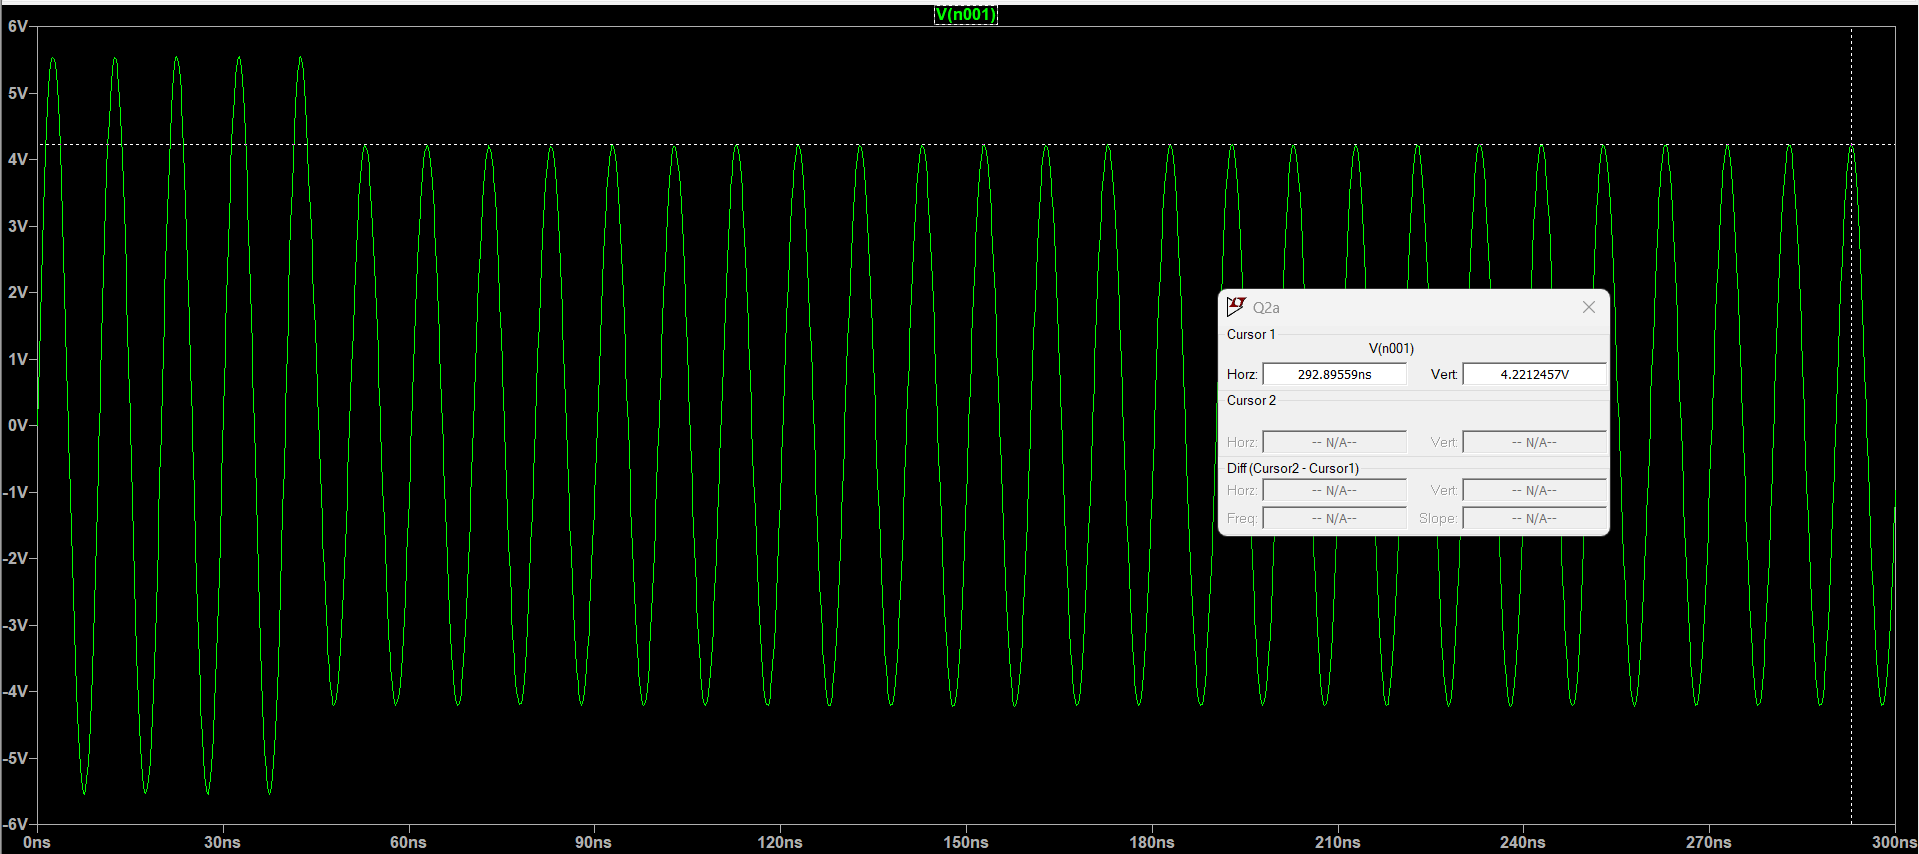
\includegraphics[scale=0.32]{2 a i.png} \\ \break
    
    $v(t,z=L),\ 0 < t < 0,3 \mu s$
    
    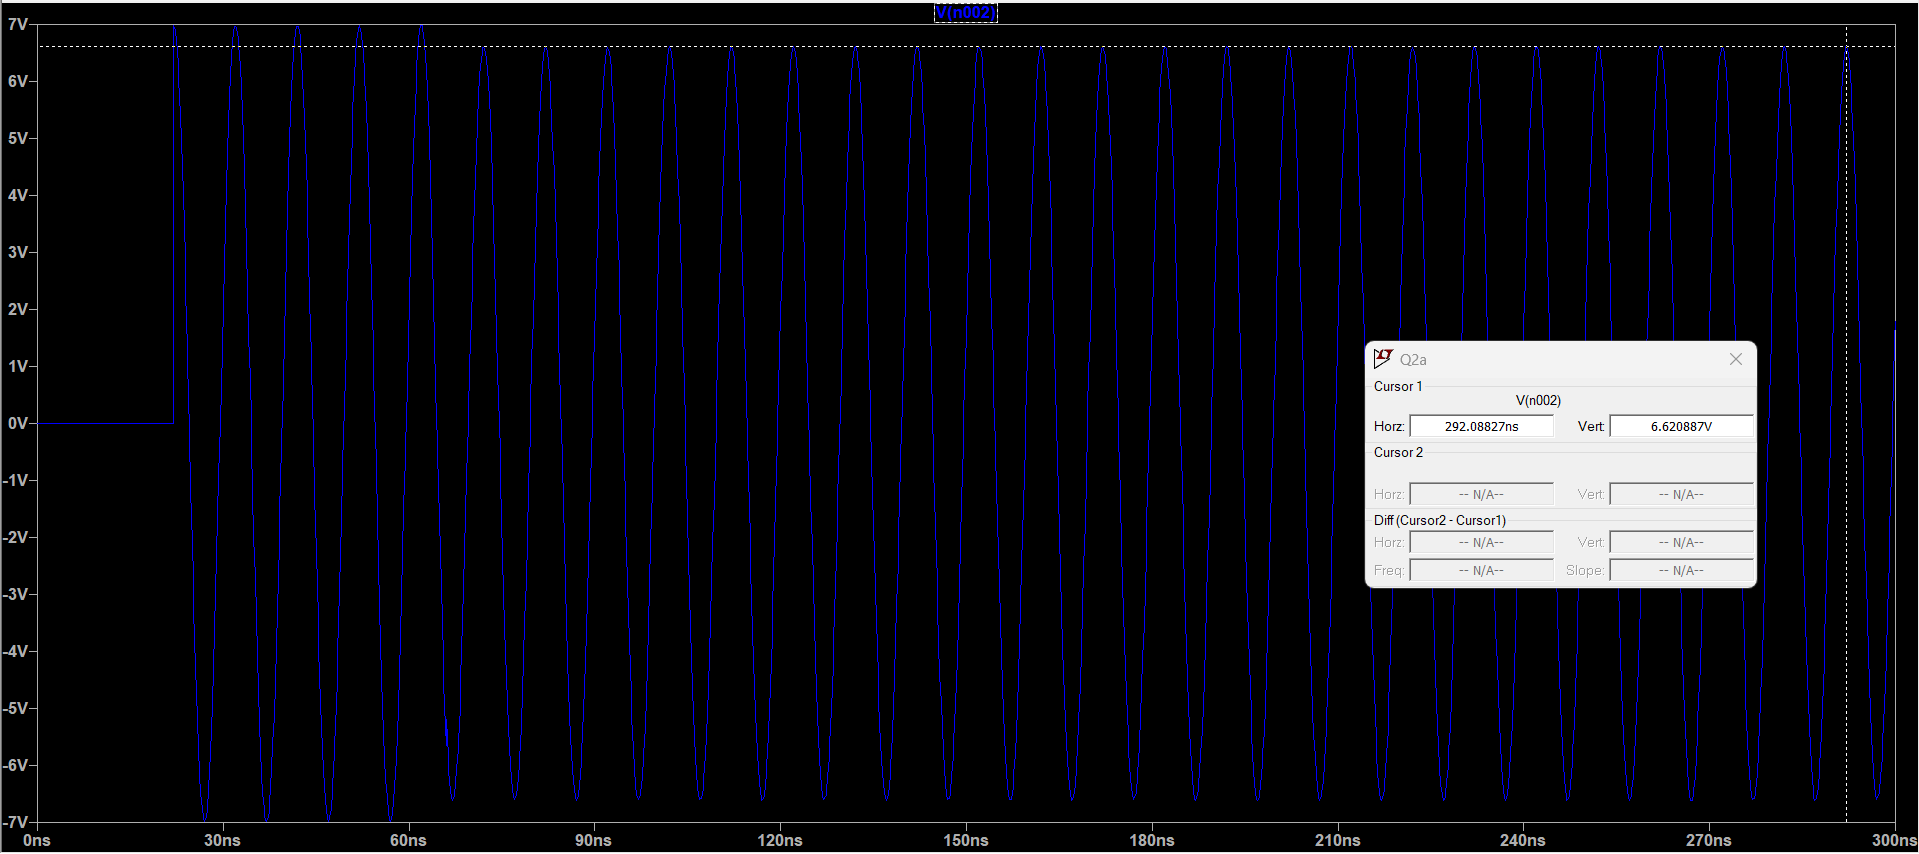
\includegraphics[scale=0.3]{2 a ii.png}
\end{center}

Observados do gráfico:

\ \ \ \ \ \ $V(z=0)_{regime}=4,213149\ V$

\ \ \ \ \ \ $V(z=L)_{regime}=6,620887\ V$


Valores esperados:

$$\rho_{ent}=\rho_L e^{-j\frac{4\pi}{\lambda}L},\ Z_{ent}=Z_0\cdot\frac{1+\rho_{ent}}{1-\rho_{ent}}$$

$$V(z=0)=Eg\cdot \frac{Z_{ent}}{Z_{ent}+R_g}$$

$$V(z=L)=V^+(0) (1+\rho_L)\ e^{-j\frac{4\pi}{\lambda}L}=V(0)\cdot \frac{1+\rho_L}{1+\rho_{ent}}\cdot e^{-j\frac{4\pi}{\lambda}L}$$

\ \ \ \ \ \ $V(z=0)_{regime} = 4,2231\ V$

\ \ \ \ \ \ $V(z=L)_{regime} = 6,6220\ V$

\paragraph{b)}

$$v(t,z=0),\ i(t,z=0),\ 30\ ns < t < 60\ ns$$

\begin{center}
    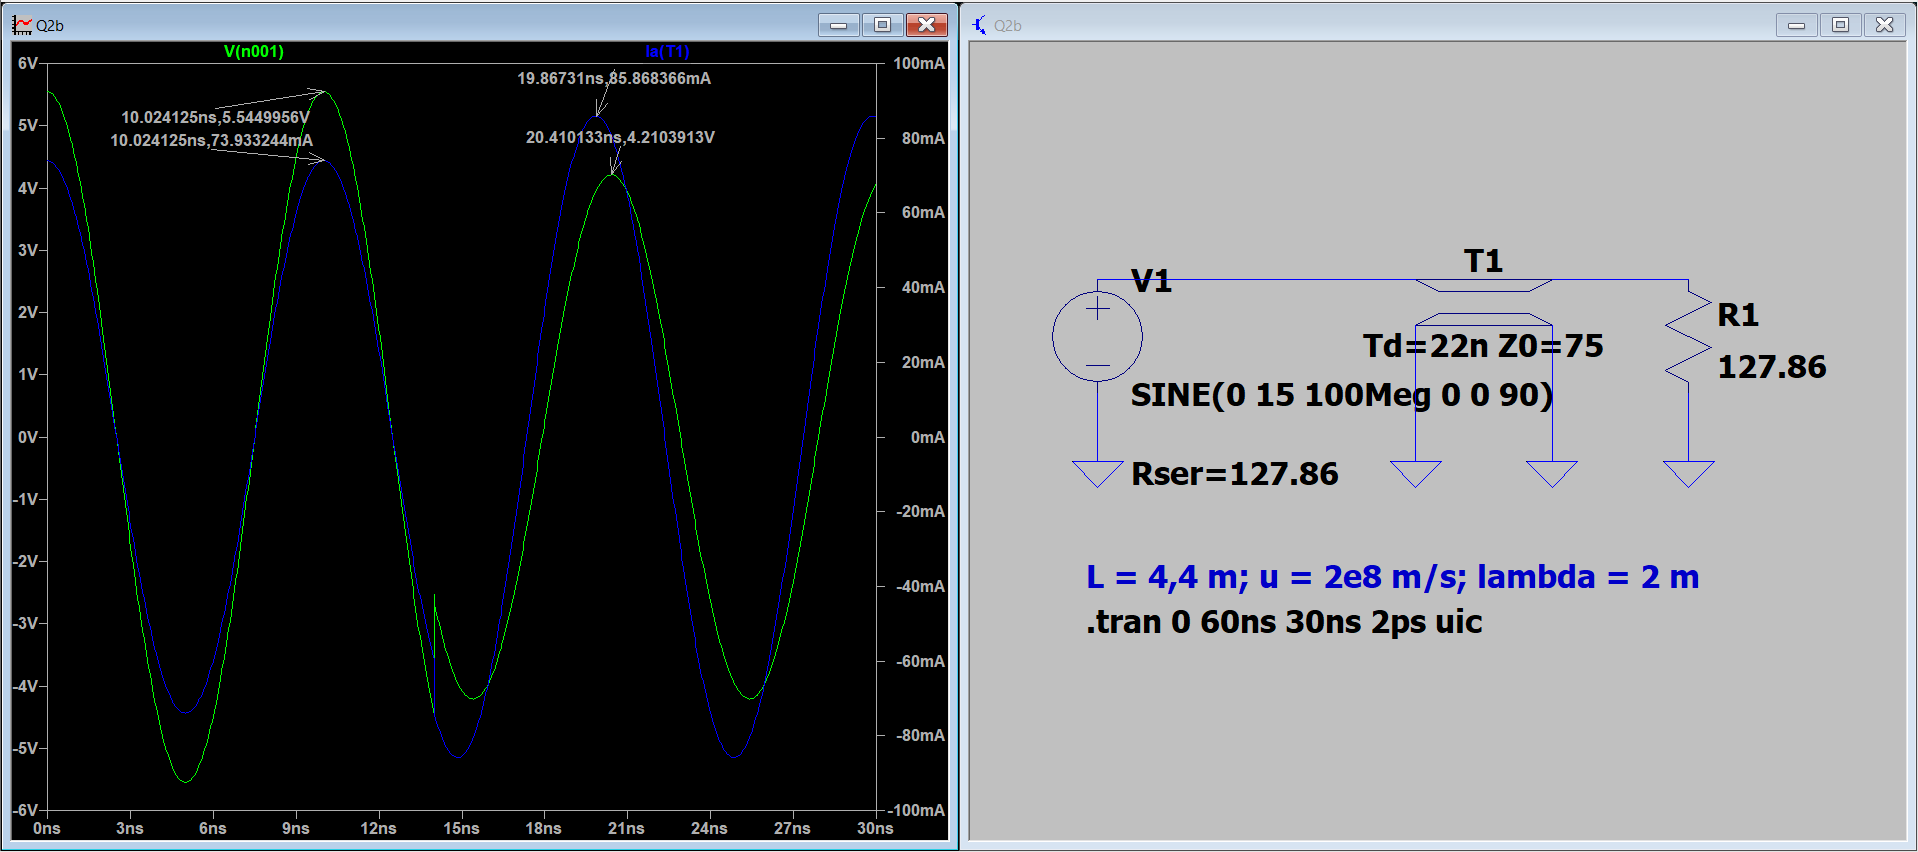
\includegraphics[scale=0.31]{2 b.png}
\end{center}

$Z_{t<44\ ns}=\frac{5,5449956\ V}{73,933244\ mA}=75,0\angle 0 \ \Omega$

$Z_{t>44\ ns}=\frac{4,2103913\ V}{85,868366\ mA}=49,033\angle -16,542^\circ \ \Omega =(46,20872 -j\ 16,40116)\ \Omega $

Calculados a partir de valores retirados dos gráficos.

A defasagem foi calculada como:

$$(19,86731-20,410133)\ ns \times 360^\circ \times 100\ MHz = -16,542^\circ$$

E a mesma tem ocorrência devido a mudança decorrida pela reflexão da onda vinda pela carga, que passou a agir neste ponto da linha neste momento, de $t=44\ ns$.

\paragraph{c)}

$$v(t,z=0),\ i(t,z=0),\ 0,28\mu s < t < 0,3 \mu s$$
\vspace{-45pt}
\begin{center}
    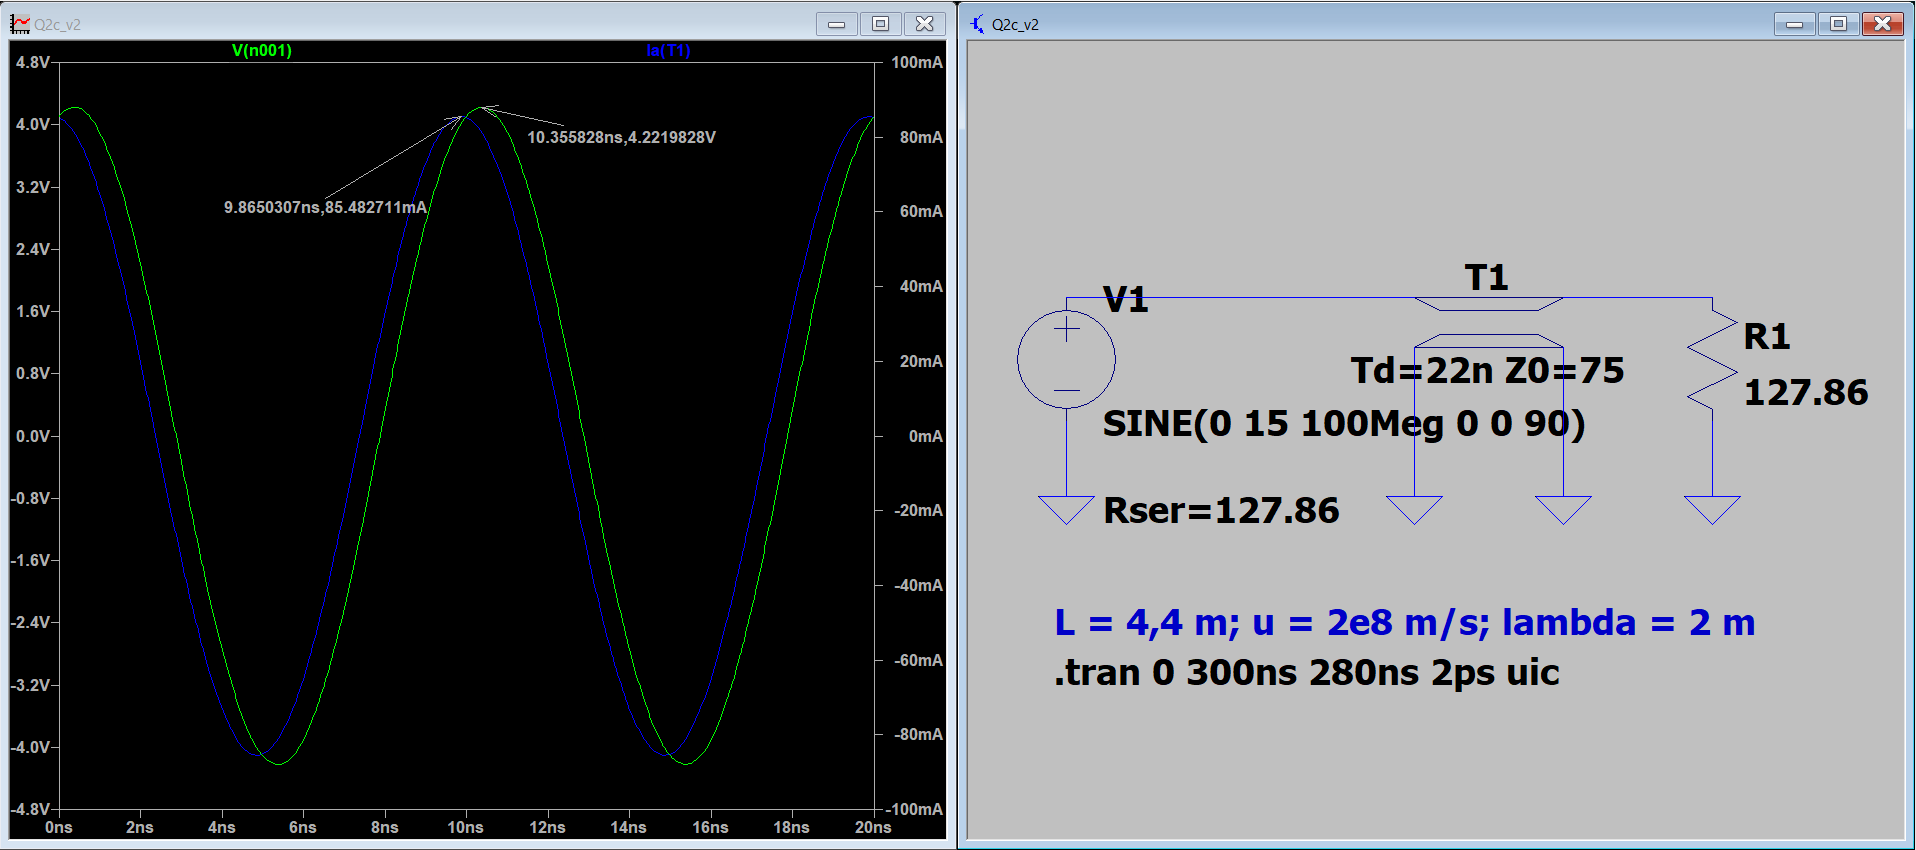
\includegraphics[scale=0.34]{2 c.png}
\end{center}

Valor observado:

\ \ \ \ \ \ $Z(z=0) =\frac{4,2219828\ V}{85,482711\ mA}= 49,39\angle -17,669^\circ \ \Omega=(47,06-j\ 14,99) \ \Omega$

Valor esperado:

\ \ \ \ \ \ $Z(z=0)= 49,403\angle -18,192^\circ \ \Omega= (46,933 - j\ 15,424) \ \Omega$

Com uma defasagem de $-0,4908 ns = -17,669^\circ$ (a 100MHz), os valores determinados a partir dos encontrados graficamente (através dos cursores) e os teóricos calculados são coerentes, ainda que a simulação não esteja perfeitamente em regime (como foi determinado pelos valores esperados) e a obtenção visual de pontos do gráfico implique em erros intrínsecos.


%%%%%%%%%%%%%%%%%%%%%%%%%%%%%%%%%%%

\newpage

\section*{Anexo - TABELA DE RESPOSTAS}

\vspace{4.5cm}


\begin{table}[h]
    \centering
    \begin{tabular}{|r|c|c|}
         \hline
         Questão & Parâmetro & Valor \\
         \hline
         1-a& $P_d=$ & 0,75 W\\
         1-b& $d_{min}=$ & 0,38 m\\
         1-c& $b=$ & 2,13 S/S\\
         1-d& $l_t=$ & 0,1397 m\\
         1-e-i& $P_{max}$ (sem toco) & -3,29297 dB \\
         ii& $P_{max}(d=d_{min})$ & 0 dB\\
         ii& $BW\ (d=d_{min})$ & 33,8 MHz\\
         iii& $P_{max}(d=3m+d_{min})$ & 0 dB\\
         iii& $BW\ (d=3m+d_{min})$ & 4,6 MHz\\
         1-f& Como muda BW? &  Para valores maiores de d,\\
         &&a largura de banda diminui\\
         &&de valor. Porém, caso o au- \\
         &&mento se dê no valor específico \\
         &&do comprimento de onda de\\
         &&cada frequência do sweep,\\
         &&o valor deve se manter igual\\
         &&ao sem esta parcela múltipla.\\
         2-a& $V_0$ - esperado & 4,2231 V\\
         & $V_0$ - observado & 4,213149 V\\
         & $V_L$ - esperado & 6,6220 V\\
         & $V_L$ - observado & 6,620887 V\\
         2-b& $Z(z=0,t<44ns)$ & $75 + j 0\ \Omega$\\
         & $Z(z=0,t>44ns)$ & $46,20872-j\ 16,40116\ \Omega $\\
         2-c& $Z(z=0;0,28\mu s<t<0,3\mu s)$ & $47,06-j\ 14,99 \ \Omega $\\
         \hline
    \end{tabular}
    \caption{Tabela de respostas}
    \label{tab:Renata}
\end{table}


%%%%%%%%%%%%%%%%%%%%%%%%%%%%%%%%%%%

\end{document}